\documentclass[12pt a4paper]{article}
\usepackage{graphicx} % Required for inserting images
\usepackage{ulem} %underline a text
\usepackage{draftwatermark} %watermark
\usepackage{soul} %for highlight
\usepackage{tikz} % For border
\usepackage[left=25mm, right=25mm, top=25mm, bottom=25mm, paper=a4paper]{geometry} % For page margins
\usetikzlibrary{shapes.geometric, positioning, calc}
\usepackage{ragged2e} % For centering
\usepackage{setspace} % For spacing between the lines
\usepackage{fancyhdr}  % For header and footer
\usepackage{moresize} % For more sizing
\usepackage{pifont} % For Times font and more bulletin options
\usepackage{tabularx}  % For tables
\usepackage{array}  % For table cell spaces
\usepackage{colortbl}  % Colouring the table
\usepackage{pgfplots} % For bar chart
\usepackage{pdflscape} % For landshape mode page
\usepackage{multicol}
% \usepackage[usegeomentry]{typearea}
% \newenvironment{landscape}{%
%     \KOMAoptions{paper=landscape, DIV=last}
%     \newgeometry{left=25mm, right=25mm, top=25mm, bottom=25mm, paper=a4paper}
%     \fancyheadoffset{0\linewidth}
% }{\clearpage}





\renewcommand{\familydefault}{\rmdefault}
\spacing{2}



\SetWatermarkAngle{39}
\SetWatermarkScale{4}
\SetWatermarkText{Learn Basics}


\pagestyle{fancy}
\fancyhf{}
\chead{ \fancyplain{} \Large \textcolor{black}{\Centering{Learn Basics \\ Report Graph} \vspace{0.5cm}}}
\fancyfoot[C]{\thepage}

\renewcommand{\headrulewidth}{1.2pt}

\pgfplotsset{width=9cm, compat=1.7}



\begin{document}

\begin{center}
\HUGE \textbf{\uline{Task 3}}
\thispagestyle{empty}
\end{center}


\newpage
\thispagestyle{empty}

\begin{tikzpicture}
[remember picture, overlay] \draw[line width=1pt]
($(current page.north west) + (0.6in, -0.6in)$) rectangle 
($(current page.south east) + (-0.6in, 0.6in)$);
\end{tikzpicture}
    
\spacing{3}
\vspace*{\stretch{1}}
\begin{center}
\begin{Huge}
\sethlcolor{yellow}
\hl{\textbf{Bar Graph}}
\end{Huge}
\end{center}
\vspace*{\stretch{1}}

\newpage


\spacing{2.5}
\begin{huge}
\noindent \LARGE \newline 
\\
\textbf{Bar graphs} are the pictorial representation of data (generally grouped), in the form of vertical or horizontal rectangular bars, where the length of bars are proportional to the measure of data. They are also known as bar charts. Bar graphs are one of the means of \textcolor{blue}{\uline{data handling}} in statistics.   \\
\end{huge}

\spacing{4.9}
\begin{huge}
\noindent \LARGE
The pictorial representation of grouped data, in the form of vertical or horizontal rectangular bars, where the lengths of the bars are equivalent to the measure of data, are known as bar graphs or bar charts. The bars drawn are of uniform width, and the variable quantity is represented on one of the axes. Also, the measure of the variable is depicted on the other axes. The heights or the lengths of the bars denote the value of the variable, and these graphs are also used to compare certain quantities. 
\end{huge}

\newpage

\hfill \break

\begin{Large}
\renewcommand{\arraystretch}{0.45}

\noindent
\centering
\begin{tabular}{|>{\centering\arraybackslash} m{3.55cm} |>{\centering\arraybackslash \columncolor{cyan!20}} m{3.55cm} |>{\centering\arraybackslash \columncolor{magenta!20}} m{3.55cm} |>{\centering\arraybackslash} m{3.55cm} |}
     \hline
     \textbf{Subject} & \textbf{Maths} & \textbf{Science 1 }& \textbf{Science 2} \\
     \hline
     A &  \ding{51}  & \ding{56}  & \ding{51}  \\
     \hline
     B  &   &   &   \\
     \hline
     C &    &   & \cellcolor{orange!20}  \\
     \hline
     D  &   &   &   \\
     \hline
     E &    &   &   \\
     \hline
     F  &   &   &   \\
     \hline
     G &    &   &   \\
     \hline
\end{tabular}

\hfill \break

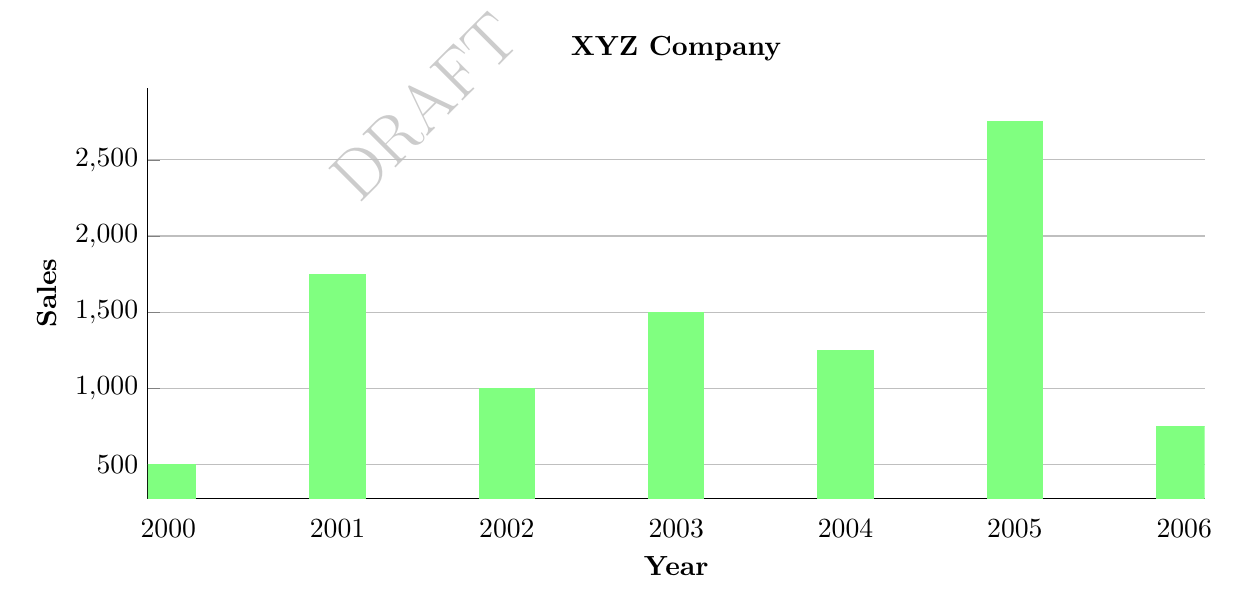
\begin{tikzpicture}
\begin{axis}[
  symbolic x coords = {2000, 2001, 2002, 2003, 2004, 2005, 2006},
  xtick = data,
  xlabel = \textbf{Year},
  ylabel = \textbf{Sales},
  ytick = {0,500,...,3000},
  ybar,
  title = {\textbf{XYZ Company}},
  height = 6.8cm,
  width = 15cm,
  bar width = 20pt,
  ymajorgrids = true,
  major x tick style = transparent,
  axis x line*=bottom,
  axis y line*=left,
  enlarge x limits=0.02
  ]
\addplot [style = {green!50, fill=green!50}]coordinates {
  (2000, 500)
  (2001, 1750)
  (2002, 1000)
  (2003, 1500)
  (2004, 1250)
  (2005, 2750)
  (2006, 750)
};
\end{axis}
\end{tikzpicture}

\end{Large}


\newpage

\hfill \break

\begin{Large}
\centering
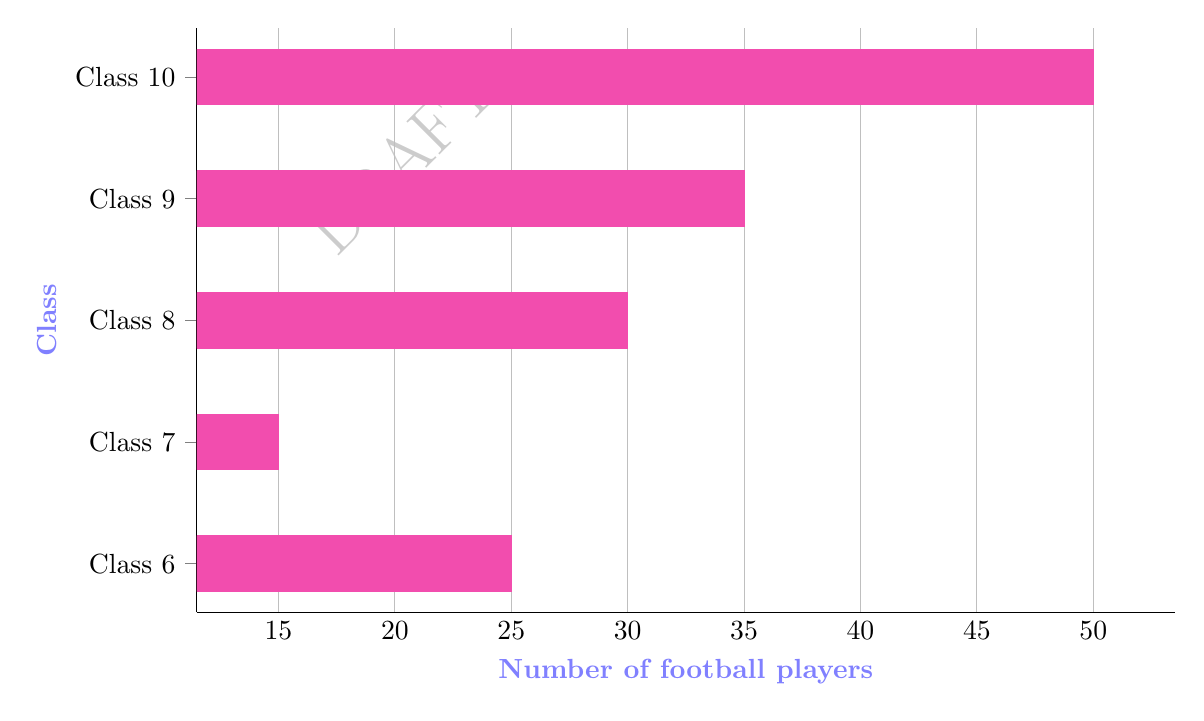
\begin{tikzpicture}
\begin{axis}[
  xbar, % this makes the bars horizontal
  xlabel = \textcolor{blue!50}{\textbf{Number of football players}}, % label for the x-axis
  symbolic y coords = {Class 6,Class 7,Class 8,Class 9,Class 10}, % labels for the y-axis
  ytick = data, % show ticks for each y coordinate
  ylabel = \textcolor{blue!50}{\textbf{Class}},
  width = 14cm,
  height = 9cm,
  bar width = 20pt,
  xmajorgrids = true,
  major x tick style = transparent,
  axis x line*=bottom,
  axis y line*=left,
  ]
\addplot [style = {magenta!70, fill=magenta!70}] coordinates {
  (25,Class 6)  
  (15,Class 7) 
  (30,Class 8) 
  (35,Class 9)
  (50,Class 10)
};
\end{axis}
\end{tikzpicture}

\vspace{3cm}

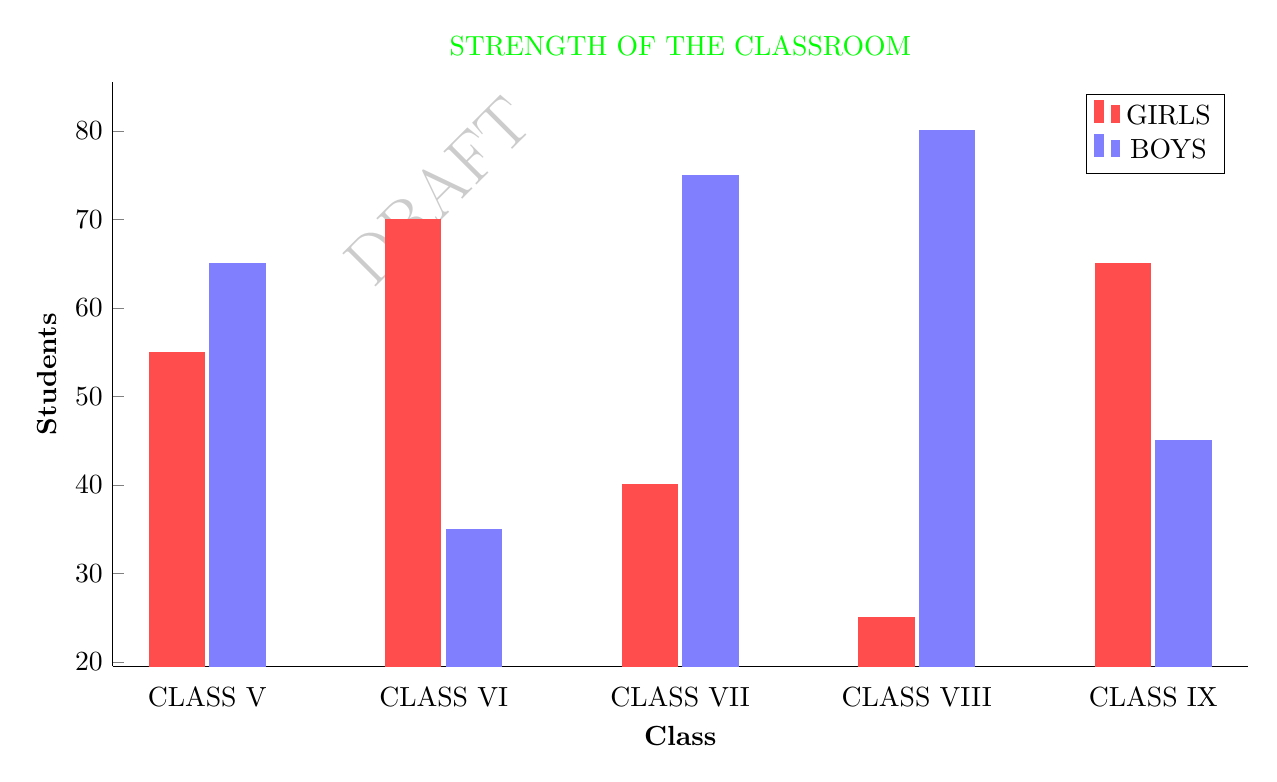
\begin{tikzpicture}
\begin{axis}[
  symbolic x coords = {CLASS V, CLASS VI, CLASS VII, CLASS VIII, CLASS IX},
  xtick = data,
  xlabel = \textbf{Class},
  ylabel = \textbf{Students},
  ytick = {0,10,...,90},
  ybar,
  title = {\textcolor{green}{STRENGTH OF THE CLASSROOM}},
  height = 9cm,
  width = 16cm,
  bar width = 20pt,
  major x tick style = transparent,
  axis x line*=bottom,
  axis y line*=left,
  ]
\addplot [style = {red!70, fill=red!70}] coordinates {
  (CLASS V, 55)
  (CLASS VI, 70)
  (CLASS VII, 40)
  (CLASS VIII, 25)
  (CLASS IX, 65)
};
\addplot [style = {blue!50, fill=blue!50}] coordinates {
  (CLASS V, 65)
  (CLASS VI, 35)
  (CLASS VII, 75)
  (CLASS VIII, 80)
  (CLASS IX, 45)
};
\legend{GIRLS, BOYS}

\end{axis}
\end{tikzpicture}

\end{Large}



\newpage
\newgeometry{left=10mm, right=10mm, top=10mm, bottom=10mm, paper=a4paper}

\begin{landscape}


\SetWatermarkAngle{130}
\thispagestyle{empty}
\spacing{1.3}
\setlength{\columnsep}{0.8cm}

\Centering{\Large Learn Basics \\ Report Graph} \\

\rule{28cm}{1pt}
\begin{multicols*}{2}

\begin{small}

\centering\textbf{\large Test Wise Performance}
\vspace{16pt}

\renewcommand{\arraystretch}{1.45}

\noindent
\centering
\begin{tabular}{|>{\centering\arraybackslash} m{0.7cm} |>{\centering\arraybackslash } m{3.55cm} |>{\centering\arraybackslash} m{2cm} |>{\centering\arraybackslash} m{2cm} |>{\centering\arraybackslash} m{1.7cm} | >{\centering\arraybackslash} m{1.7cm}|}
     \hline
     \textbf{S.No} & \textbf{Topic Name} & \textbf{Performance with Absentees }& \textbf{Performance without Absentees} & \textbf{Attempted} & \textbf{Yet to Attempted} \\
     \hline
     1 &  Adolescence and puberty  & \cellcolor{magenta!20}{25\%} & \cellcolor{magenta!20}{38\%} & 4 & 2 \\
     \hline
     2  & Changes during puberty  & \cellcolor{magenta!20}{31\%}  &  50\% & 4 & 2 \\
     \hline
     3 &  Role of hormones  & \cellcolor{magenta!20}{23\%}  &  47\% & 3 & 3 \\
     \hline
     4  & Reproductive phase of humans  & \cellcolor{magenta!20}{28\% } & 56\% & 3 & 3  \\
     \hline
     5 & Determination of the sex of the baby   &  \cellcolor{magenta!20}{33\%} &  67\% & 3 & 3 \\
     \hline
     6  & Reproductive health  & \cellcolor{magenta!20}{10\%}  & \cellcolor{magenta!20}{31\%} & 2 & 4  \\
     \hline
\end{tabular} \\


\vspace{28pt}
\centering\textbf{\large Concepts need to be revised}

\begin{multicols*}{2}
\begin{enumerate}
    \item Adolescence and puberty
    \item Increase in height
    \item Change in body shape
    \item Voice change
    \item Development of mammary glands 
    \item Development of sex organs 
    \item Reaching mental, intellectual maturity 
    \item Secondary sexual characters 
    \item Role of hormones in initiating reproductive function 
    \item Hormones other than sex hormones 
    \item Reproductive phase of life in humans 
    \item How is sex baby determined?  
    \item Boys' changes during adolescence  
    \item Menstrual cycle  
    \item Reproductive health  
    \item Personal hygiene   
    \item Physical exercise   
    \item Say no drugs
\end{enumerate}
    
\end{multicols*}




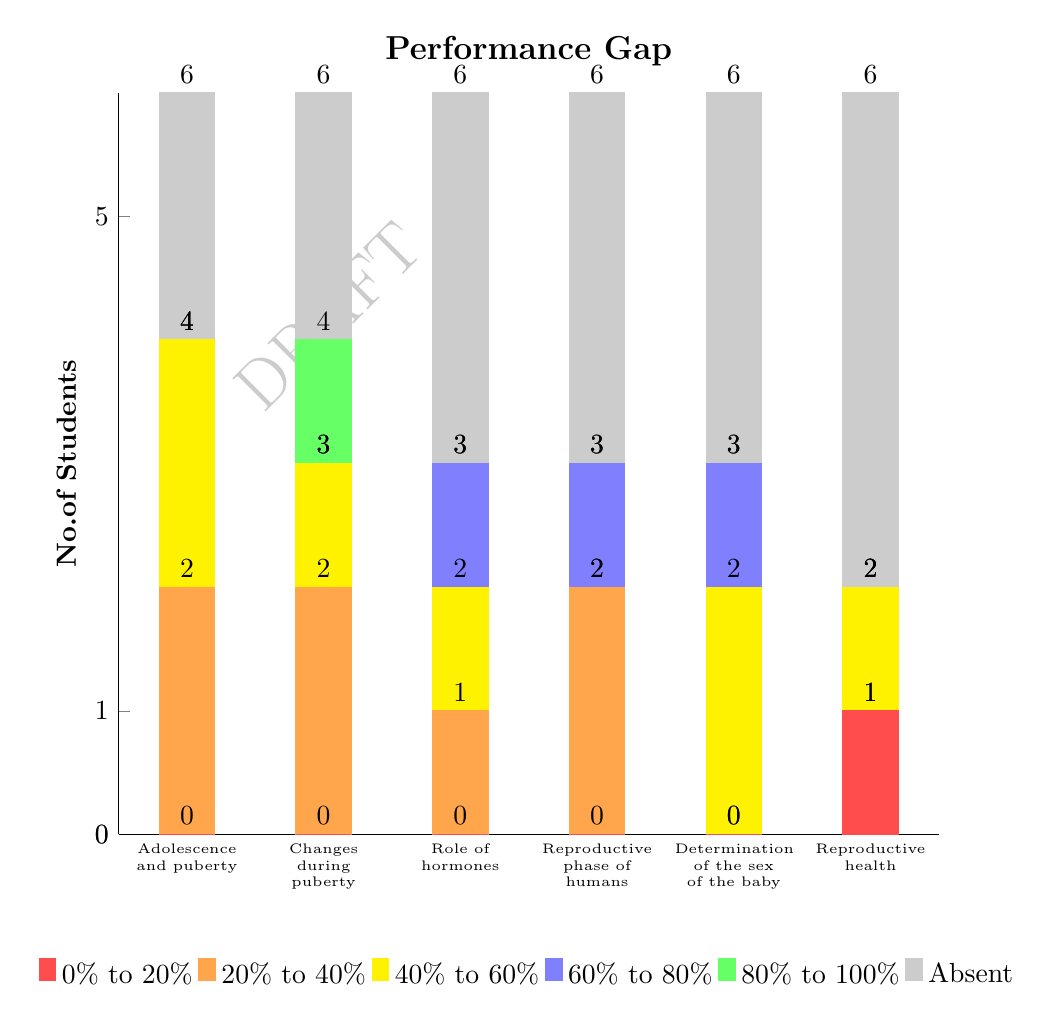
\begin{tikzpicture}
\begin{axis}[
  symbolic x coords = {Adolescence and puberty, Changes during puberty, Role of hormones, Reproductive phase of humans, Determination of the sex of the baby, Reproductive health},
  xtick = data,
  ylabel = \textbf{No.of Students},
  ytick = {0,1,.,5},
  ybar stacked,
  title = {\textbf{\large Performance Gap}},
  height = 11cm,
  width = 12cm,
  bar width = 20pt,
  major x tick style = transparent,
  nodes near coords,
  nodes near coords style={color=black},
  axis x line*=bottom,
  axis y line*=left,
  enlarge y limits=0,
  legend style = {
    at={(0.5,-0.15)},
    anchor=north,
    legend columns=-1,
    inner sep=4pt,
    draw=none,
    % font=\tiny
  },
  x tick label style={font=\tiny,text width=1.5cm,align=center}
  ]
\addplot [style = {red!70, fill=red!70}] coordinates {
  (Adolescence and puberty, 0)
  (Changes during puberty, 0)
  (Role of hormones, 0)
  (Reproductive phase of humans, 0)
  (Determination of the sex of the baby, 0)
  (Reproductive health, 1)
};
\addplot [style = {orange!70, fill=orange!70}] coordinates {
  (Adolescence and puberty, 2)
  (Changes during puberty, 2)
  (Role of hormones, 1)
  (Reproductive phase of humans, 2)
  (Determination of the sex of the baby, 0)
  (Reproductive health, 0)
};
\addplot [style = {yellow, fill=yellow}] coordinates {
  (Adolescence and puberty, 2)
  (Changes during puberty, 1)
  (Role of hormones, 1)
  (Reproductive phase of humans, 0)
  (Determination of the sex of the baby, 2)
  (Reproductive health, 1)
};
\addplot [style = {blue!50, fill=blue!50}] coordinates {
  (Adolescence and puberty, 0)
  (Changes during puberty, 0)
  (Role of hormones, 1)
  (Reproductive phase of humans, 1)
  (Determination of the sex of the baby, 1)
  (Reproductive health, 0)
};
\addplot [style = {green!60, fill=green!60}] coordinates {
  (Adolescence and puberty, 0)
  (Changes during puberty, 1)
  (Role of hormones, 0)
  (Reproductive phase of humans, 0)
  (Determination of the sex of the baby, 0)
  (Reproductive health, 0)
};
\addplot [style = {black!20, fill=black!20}] coordinates {
  (Adolescence and puberty, 2)
  (Changes during puberty, 2)
  (Role of hormones, 3)
  (Reproductive phase of humans, 3)
  (Determination of the sex of the baby, 3)
  (Reproductive health, 4)
};
\legend{0\% to 20\%, 20\% to 40\%, 40\% to 60\%, 60\% to 80\%, 80\% to 100\%, Absent}

\end{axis}
\end{tikzpicture}

\end{small}


\end{multicols*}

\end{landscape}

\restoregeometry

\newpage

\begin{tikzpicture}
    \begin{axis}[
        title={Test Consumption in \%},
        xlabel={Month},
        ylabel={Percentage},
        xmin=0, xmax=5,
        ymin=50, ymax=90,
        xtick={1,2,3,4},
        xticklabels={June, July, August, September},
        ytick={60,70,80,90},
        legend pos=south east,
        ymajorgrids=true,
        grid style=dashed,
    ]
    
    \addplot[
        color=blue,
        mark=square,
    ]
    coordinates {
        (1,86)(2,81)(3,80)(4,77)
    };
         
    \addplot[
        color=green,
        mark=*,
    ]
    coordinates {
        (1,80)(2,77)(3.5)
    };
    \legend{Math, Science}
    \end{axis}
\end{tikzpicture}




\end{document}